% Options for packages loaded elsewhere
\PassOptionsToPackage{unicode}{hyperref}
\PassOptionsToPackage{hyphens}{url}
%
\documentclass[
]{article}
\usepackage{lmodern}
\usepackage{amsmath}
\usepackage{ifxetex,ifluatex}
\ifnum 0\ifxetex 1\fi\ifluatex 1\fi=0 % if pdftex
  \usepackage[T1]{fontenc}
  \usepackage[utf8]{inputenc}
  \usepackage{textcomp} % provide euro and other symbols
  \usepackage{amssymb}
\else % if luatex or xetex
  \usepackage{unicode-math}
  \defaultfontfeatures{Scale=MatchLowercase}
  \defaultfontfeatures[\rmfamily]{Ligatures=TeX,Scale=1}
\fi
% Use upquote if available, for straight quotes in verbatim environments
\IfFileExists{upquote.sty}{\usepackage{upquote}}{}
\IfFileExists{microtype.sty}{% use microtype if available
  \usepackage[]{microtype}
  \UseMicrotypeSet[protrusion]{basicmath} % disable protrusion for tt fonts
}{}
\makeatletter
\@ifundefined{KOMAClassName}{% if non-KOMA class
  \IfFileExists{parskip.sty}{%
    \usepackage{parskip}
  }{% else
    \setlength{\parindent}{0pt}
    \setlength{\parskip}{6pt plus 2pt minus 1pt}}
}{% if KOMA class
  \KOMAoptions{parskip=half}}
\makeatother
\usepackage{xcolor}
\IfFileExists{xurl.sty}{\usepackage{xurl}}{} % add URL line breaks if available
\IfFileExists{bookmark.sty}{\usepackage{bookmark}}{\usepackage{hyperref}}
\hypersetup{
  pdftitle={PAD-ATA Call Log Analysis},
  hidelinks,
  pdfcreator={LaTeX via pandoc}}
\urlstyle{same} % disable monospaced font for URLs
\usepackage[margin=1in]{geometry}
\usepackage{color}
\usepackage{fancyvrb}
\newcommand{\VerbBar}{|}
\newcommand{\VERB}{\Verb[commandchars=\\\{\}]}
\DefineVerbatimEnvironment{Highlighting}{Verbatim}{commandchars=\\\{\}}
% Add ',fontsize=\small' for more characters per line
\usepackage{framed}
\definecolor{shadecolor}{RGB}{248,248,248}
\newenvironment{Shaded}{\begin{snugshade}}{\end{snugshade}}
\newcommand{\AlertTok}[1]{\textcolor[rgb]{0.94,0.16,0.16}{#1}}
\newcommand{\AnnotationTok}[1]{\textcolor[rgb]{0.56,0.35,0.01}{\textbf{\textit{#1}}}}
\newcommand{\AttributeTok}[1]{\textcolor[rgb]{0.77,0.63,0.00}{#1}}
\newcommand{\BaseNTok}[1]{\textcolor[rgb]{0.00,0.00,0.81}{#1}}
\newcommand{\BuiltInTok}[1]{#1}
\newcommand{\CharTok}[1]{\textcolor[rgb]{0.31,0.60,0.02}{#1}}
\newcommand{\CommentTok}[1]{\textcolor[rgb]{0.56,0.35,0.01}{\textit{#1}}}
\newcommand{\CommentVarTok}[1]{\textcolor[rgb]{0.56,0.35,0.01}{\textbf{\textit{#1}}}}
\newcommand{\ConstantTok}[1]{\textcolor[rgb]{0.00,0.00,0.00}{#1}}
\newcommand{\ControlFlowTok}[1]{\textcolor[rgb]{0.13,0.29,0.53}{\textbf{#1}}}
\newcommand{\DataTypeTok}[1]{\textcolor[rgb]{0.13,0.29,0.53}{#1}}
\newcommand{\DecValTok}[1]{\textcolor[rgb]{0.00,0.00,0.81}{#1}}
\newcommand{\DocumentationTok}[1]{\textcolor[rgb]{0.56,0.35,0.01}{\textbf{\textit{#1}}}}
\newcommand{\ErrorTok}[1]{\textcolor[rgb]{0.64,0.00,0.00}{\textbf{#1}}}
\newcommand{\ExtensionTok}[1]{#1}
\newcommand{\FloatTok}[1]{\textcolor[rgb]{0.00,0.00,0.81}{#1}}
\newcommand{\FunctionTok}[1]{\textcolor[rgb]{0.00,0.00,0.00}{#1}}
\newcommand{\ImportTok}[1]{#1}
\newcommand{\InformationTok}[1]{\textcolor[rgb]{0.56,0.35,0.01}{\textbf{\textit{#1}}}}
\newcommand{\KeywordTok}[1]{\textcolor[rgb]{0.13,0.29,0.53}{\textbf{#1}}}
\newcommand{\NormalTok}[1]{#1}
\newcommand{\OperatorTok}[1]{\textcolor[rgb]{0.81,0.36,0.00}{\textbf{#1}}}
\newcommand{\OtherTok}[1]{\textcolor[rgb]{0.56,0.35,0.01}{#1}}
\newcommand{\PreprocessorTok}[1]{\textcolor[rgb]{0.56,0.35,0.01}{\textit{#1}}}
\newcommand{\RegionMarkerTok}[1]{#1}
\newcommand{\SpecialCharTok}[1]{\textcolor[rgb]{0.00,0.00,0.00}{#1}}
\newcommand{\SpecialStringTok}[1]{\textcolor[rgb]{0.31,0.60,0.02}{#1}}
\newcommand{\StringTok}[1]{\textcolor[rgb]{0.31,0.60,0.02}{#1}}
\newcommand{\VariableTok}[1]{\textcolor[rgb]{0.00,0.00,0.00}{#1}}
\newcommand{\VerbatimStringTok}[1]{\textcolor[rgb]{0.31,0.60,0.02}{#1}}
\newcommand{\WarningTok}[1]{\textcolor[rgb]{0.56,0.35,0.01}{\textbf{\textit{#1}}}}
\usepackage{graphicx}
\makeatletter
\def\maxwidth{\ifdim\Gin@nat@width>\linewidth\linewidth\else\Gin@nat@width\fi}
\def\maxheight{\ifdim\Gin@nat@height>\textheight\textheight\else\Gin@nat@height\fi}
\makeatother
% Scale images if necessary, so that they will not overflow the page
% margins by default, and it is still possible to overwrite the defaults
% using explicit options in \includegraphics[width, height, ...]{}
\setkeys{Gin}{width=\maxwidth,height=\maxheight,keepaspectratio}
% Set default figure placement to htbp
\makeatletter
\def\fps@figure{htbp}
\makeatother
\setlength{\emergencystretch}{3em} % prevent overfull lines
\providecommand{\tightlist}{%
  \setlength{\itemsep}{0pt}\setlength{\parskip}{0pt}}
\setcounter{secnumdepth}{-\maxdimen} % remove section numbering
\ifluatex
  \usepackage{selnolig}  % disable illegal ligatures
\fi

\title{PAD-ATA Call Log Analysis}
\author{}
\date{\vspace{-2.5em}}

\begin{document}
\maketitle

\hypertarget{libraries-used-in-the-project-and-uploading-data}{%
\paragraph{Libraries used in the Project and uploading
data}\label{libraries-used-in-the-project-and-uploading-data}}

\begin{Shaded}
\begin{Highlighting}[]
\FunctionTok{library}\NormalTok{(tidyverse)}
\end{Highlighting}
\end{Shaded}

\begin{verbatim}
## -- Attaching packages ------------------------------------------------------------ tidyverse 1.3.0 --
\end{verbatim}

\begin{verbatim}
## v ggplot2 3.3.3     v purrr   0.3.4
## v tibble  3.0.3     v dplyr   1.0.2
## v tidyr   1.1.2     v stringr 1.4.0
## v readr   1.4.0     v forcats 0.5.0
\end{verbatim}

\begin{verbatim}
## -- Conflicts --------------------------------------------------------------- tidyverse_conflicts() --
## x dplyr::filter() masks stats::filter()
## x dplyr::lag()    masks stats::lag()
\end{verbatim}

\begin{Shaded}
\begin{Highlighting}[]
\FunctionTok{library}\NormalTok{(dplyr)}
\FunctionTok{library}\NormalTok{(stringr)}
\FunctionTok{library}\NormalTok{(svMisc)}
\end{Highlighting}
\end{Shaded}

\begin{verbatim}
## 
## Attaching package: 'svMisc'
\end{verbatim}

\begin{verbatim}
## The following object is masked from 'package:utils':
## 
##     ?
\end{verbatim}

\begin{Shaded}
\begin{Highlighting}[]
\FunctionTok{library}\NormalTok{(ggplot2)}
\FunctionTok{library}\NormalTok{(gtable)}
\FunctionTok{library}\NormalTok{(}\StringTok{"ggpubr"}\NormalTok{)}

\NormalTok{log\_data }\OtherTok{\textless{}{-}} \FunctionTok{read\_csv}\NormalTok{(}\StringTok{"\textasciitilde{}/Desktop/PAE/github/data/logData.csv"}\NormalTok{)}
\end{Highlighting}
\end{Shaded}

\begin{verbatim}
## 
## -- Column specification -----------------------------------------------------------------------------
## cols(
##   callerId = col_double(),
##   langId = col_double(),
##   callTime = col_datetime(format = ""),
##   lastCallTime = col_character(),
##   noCallsMade = col_double(),
##   noContentListened = col_double(),
##   callId = col_character(),
##   eventTime = col_datetime(format = ""),
##   logInfo = col_character(),
##   logInfoId = col_double(),
##   inSurvey = col_logical()
## )
\end{verbatim}

\begin{Shaded}
\begin{Highlighting}[]
\CommentTok{\#MAKE IT ALL UPPER!!!}

\NormalTok{log\_data}\SpecialCharTok{$}\NormalTok{logInfo }\OtherTok{\textless{}{-}} \FunctionTok{toupper}\NormalTok{(log\_data}\SpecialCharTok{$}\NormalTok{logInfo)}

\DocumentationTok{\#\#\# GETTING THE DATE MONTH AND YEAR IF I WANT!!!}
\NormalTok{extractdate }\OtherTok{\textless{}{-}} \ControlFlowTok{function}\NormalTok{(date) \{}
\NormalTok{    day }\OtherTok{\textless{}{-}} \FunctionTok{format}\NormalTok{(date, }\AttributeTok{format=}\StringTok{"\%d"}\NormalTok{)}
\NormalTok{    month }\OtherTok{\textless{}{-}} \FunctionTok{format}\NormalTok{(date, }\AttributeTok{format=}\StringTok{"\%m"}\NormalTok{)}
\NormalTok{    year }\OtherTok{\textless{}{-}} \FunctionTok{format}\NormalTok{(date, }\AttributeTok{format=}\StringTok{"\%Y"}\NormalTok{)}

    \FunctionTok{cbind}\NormalTok{(day, month, year)}
\NormalTok{\}}

\CommentTok{\#making first calls}
\NormalTok{first\_call}\OtherTok{\textless{}{-}}\FunctionTok{extractdate}\NormalTok{(log\_data}\SpecialCharTok{$}\NormalTok{callTime)}


\CommentTok{\#making last call}
\NormalTok{last\_day }\OtherTok{\textless{}{-}}\FunctionTok{substr}\NormalTok{(log\_data}\SpecialCharTok{$}\NormalTok{lastCallTime, }\DecValTok{9}\NormalTok{, }\DecValTok{10}\NormalTok{)}
\NormalTok{last\_month }\OtherTok{\textless{}{-}} \FunctionTok{substr}\NormalTok{(log\_data}\SpecialCharTok{$}\NormalTok{lastCallTime, }\DecValTok{6}\NormalTok{, }\DecValTok{7}\NormalTok{)}
\NormalTok{last\_year }\OtherTok{\textless{}{-}}\FunctionTok{substr}\NormalTok{(log\_data}\SpecialCharTok{$}\NormalTok{lastCallTime, }\DecValTok{1}\NormalTok{, }\DecValTok{4}\NormalTok{)}

\NormalTok{log\_data}\OtherTok{\textless{}{-}}\FunctionTok{cbind}\NormalTok{(log\_data, first\_call,last\_day,last\_month,last\_year)}

\CommentTok{\#Converting columns to numeric}
\NormalTok{log\_data}\SpecialCharTok{$}\NormalTok{day }\OtherTok{\textless{}{-}}\FunctionTok{as.numeric}\NormalTok{(log\_data}\SpecialCharTok{$}\NormalTok{day)}
\NormalTok{log\_data}\SpecialCharTok{$}\NormalTok{last\_day }\OtherTok{\textless{}{-}} \FunctionTok{as.numeric}\NormalTok{(log\_data}\SpecialCharTok{$}\NormalTok{last\_day)}
\end{Highlighting}
\end{Shaded}

\begin{verbatim}
## Warning: NAs introduced by coercion
\end{verbatim}

\begin{Shaded}
\begin{Highlighting}[]
\NormalTok{log\_data}\SpecialCharTok{$}\NormalTok{month }\OtherTok{\textless{}{-}}\FunctionTok{as.numeric}\NormalTok{(log\_data}\SpecialCharTok{$}\NormalTok{month)}
\NormalTok{log\_data}\SpecialCharTok{$}\NormalTok{last\_month }\OtherTok{\textless{}{-}} \FunctionTok{as.numeric}\NormalTok{(log\_data}\SpecialCharTok{$}\NormalTok{last\_month)}
\end{Highlighting}
\end{Shaded}

\begin{verbatim}
## Warning: NAs introduced by coercion
\end{verbatim}

\begin{Shaded}
\begin{Highlighting}[]
\NormalTok{log\_data}\SpecialCharTok{$}\NormalTok{year }\OtherTok{\textless{}{-}} \FunctionTok{as.numeric}\NormalTok{(log\_data}\SpecialCharTok{$}\NormalTok{year)}
\NormalTok{log\_data}\SpecialCharTok{$}\NormalTok{last\_year }\OtherTok{\textless{}{-}} \FunctionTok{as.numeric}\NormalTok{(log\_data}\SpecialCharTok{$}\NormalTok{last\_year )}
\end{Highlighting}
\end{Shaded}

\begin{verbatim}
## Warning: NAs introduced by coercion
\end{verbatim}

\begin{Shaded}
\begin{Highlighting}[]
\NormalTok{log\_data}\SpecialCharTok{$}\NormalTok{year }\OtherTok{\textless{}{-}}\NormalTok{ log\_data}\SpecialCharTok{$}\NormalTok{year }\SpecialCharTok{+}\NormalTok{log\_data}\SpecialCharTok{$}\NormalTok{month}\SpecialCharTok{/}\DecValTok{12}
\NormalTok{log\_data}\SpecialCharTok{$}\NormalTok{last\_year }\OtherTok{\textless{}{-}}\NormalTok{ log\_data}\SpecialCharTok{$}\NormalTok{last\_year }\SpecialCharTok{+}\NormalTok{ log\_data}\SpecialCharTok{$}\NormalTok{last\_month}\SpecialCharTok{/}\DecValTok{12}

\NormalTok{log\_data}\SpecialCharTok{$}\NormalTok{caller\_lifetime }\OtherTok{\textless{}{-}}\NormalTok{ log\_data}\SpecialCharTok{$}\NormalTok{last\_year }\SpecialCharTok{{-}}\NormalTok{ log\_data}\SpecialCharTok{$}\NormalTok{year}
\end{Highlighting}
\end{Shaded}

\emph{Cmd+Option+I}.

\emph{Cmd+Shift+K}

\hypertarget{preliminary-distributions}{%
\subsubsection{PRELIMINARY
DISTRIBUTIONS}\label{preliminary-distributions}}

\textbf{In this section, we display some of the basic distributions of
the data including languages, total lifeetime of a given caller, colls
made, content accessed, and the ratio of content listened to calls
made.}

\textbf{Based on the graphs below, we are nervous that some of the data
is not random given the incredibly high ratio for content listened to
calls made, but given that the data is distributed fairly evenly across
thee different graphs, we are unsure}

\begin{Shaded}
\begin{Highlighting}[]
\NormalTok{lang\_spoken }\OtherTok{\textless{}{-}}\NormalTok{ log\_data }\SpecialCharTok{\%\textgreater{}\%}
  \FunctionTok{group\_by}\NormalTok{(callerId, langId) }\SpecialCharTok{\%\textgreater{}\%}
  \FunctionTok{count}\NormalTok{()}

\CommentTok{\#Ditribution of languages spoken}
\FunctionTok{ggplot}\NormalTok{(}\AttributeTok{data=}\NormalTok{lang\_spoken, }\FunctionTok{aes}\NormalTok{(}\AttributeTok{x=}\NormalTok{langId)) }\SpecialCharTok{+}
  \FunctionTok{geom\_bar}\NormalTok{()}\SpecialCharTok{+}
  \FunctionTok{labs}\NormalTok{(}
    \AttributeTok{title =} \StringTok{\textquotesingle{}Distribution of Languages}
\StringTok{    1 = Amharic, 2=Oromiffa, 3=Tigrigna, 4=Wolayitta, and 5=Sidamigna\textquotesingle{}}\NormalTok{,}
    \AttributeTok{x =} \StringTok{\textquotesingle{}Language\textquotesingle{}}\NormalTok{,}
    \AttributeTok{y=} \StringTok{\textquotesingle{}count\textquotesingle{}}
\NormalTok{  )}
\end{Highlighting}
\end{Shaded}

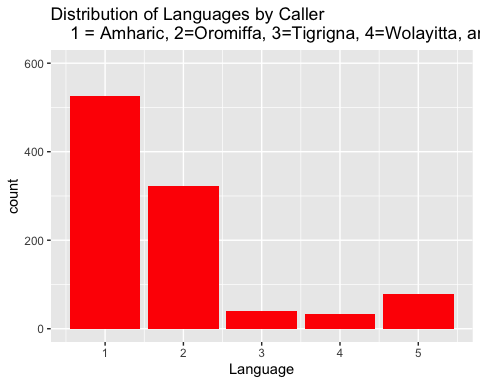
\includegraphics{pad_files/figure-latex/unnamed-chunk-2-1.pdf}

\begin{Shaded}
\begin{Highlighting}[]
\CommentTok{\#Ditribution otiem difference beetween firs tand last call}

\NormalTok{lifetime}\OtherTok{\textless{}{-}}\NormalTok{ log\_data }\SpecialCharTok{\%\textgreater{}\%}
  \FunctionTok{group\_by}\NormalTok{(callerId, caller\_lifetime) }\SpecialCharTok{\%\textgreater{}\%}
  \FunctionTok{count}\NormalTok{()}

\FunctionTok{ggplot}\NormalTok{(}\AttributeTok{data=}\NormalTok{lifetime, }\FunctionTok{aes}\NormalTok{(}\AttributeTok{x=}\NormalTok{caller\_lifetime)) }\SpecialCharTok{+}
  \FunctionTok{geom\_histogram}\NormalTok{(}\AttributeTok{fill=}\StringTok{\textquotesingle{}brown\textquotesingle{}}\NormalTok{, }\AttributeTok{color=}\StringTok{\textquotesingle{}black\textquotesingle{}}\NormalTok{)}\SpecialCharTok{+}
  \FunctionTok{labs}\NormalTok{(}
    \AttributeTok{title =} \StringTok{\textquotesingle{}Distribution of Call Lifetimes\textquotesingle{}}\NormalTok{,}
    \AttributeTok{x =} \StringTok{\textquotesingle{}Years between First and Last Call\textquotesingle{}}\NormalTok{,}
    \AttributeTok{y=} \StringTok{\textquotesingle{}count\textquotesingle{}}
\NormalTok{  )}
\end{Highlighting}
\end{Shaded}

\begin{verbatim}
## `stat_bin()` using `bins = 30`. Pick better value with `binwidth`.
\end{verbatim}

\begin{verbatim}
## Warning: Removed 17 rows containing non-finite values (stat_bin).
\end{verbatim}

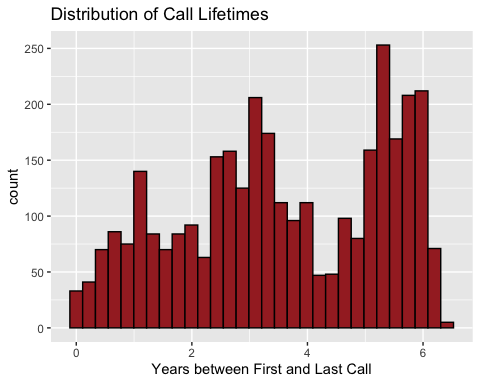
\includegraphics{pad_files/figure-latex/unnamed-chunk-2-2.pdf}

\begin{Shaded}
\begin{Highlighting}[]
\CommentTok{\#distribution of calls made}

\NormalTok{calls\_made }\OtherTok{\textless{}{-}}\NormalTok{ log\_data }\SpecialCharTok{\%\textgreater{}\%}
  \FunctionTok{group\_by}\NormalTok{(callerId, noCallsMade) }\SpecialCharTok{\%\textgreater{}\%}
  \FunctionTok{count}\NormalTok{()}

\FunctionTok{ggplot}\NormalTok{(calls\_made, }\FunctionTok{aes}\NormalTok{(}\AttributeTok{x=}\NormalTok{noCallsMade)) }\SpecialCharTok{+}
  \FunctionTok{geom\_histogram}\NormalTok{(}\AttributeTok{color=}\StringTok{"black"}\NormalTok{, }\AttributeTok{fill=}\StringTok{"blue"}\NormalTok{) }\SpecialCharTok{+}
  \FunctionTok{xlim}\NormalTok{(}\DecValTok{0}\NormalTok{,}\DecValTok{350}\NormalTok{) }\SpecialCharTok{+}
  \FunctionTok{labs}\NormalTok{(}
    \AttributeTok{title =} \StringTok{\textquotesingle{}Distribution of calls made per individual (Outliers Excluded) }\SpecialCharTok{\textbackslash{}n}
\StringTok{Min. 1st Qu.  Median  Mean   3rd Qu.    Max. }
\StringTok{    3.0    45.0    69.0     99.9    106.0    7110.0 \textquotesingle{}}\NormalTok{,}
    \AttributeTok{x =} \StringTok{\textquotesingle{}Total number of calls\textquotesingle{}}
\NormalTok{  )}
\end{Highlighting}
\end{Shaded}

\begin{verbatim}
## `stat_bin()` using `bins = 30`. Pick better value with `binwidth`.
\end{verbatim}

\begin{verbatim}
## Warning: Removed 17 rows containing non-finite values (stat_bin).
\end{verbatim}

\begin{verbatim}
## Warning: Removed 2 rows containing missing values (geom_bar).
\end{verbatim}

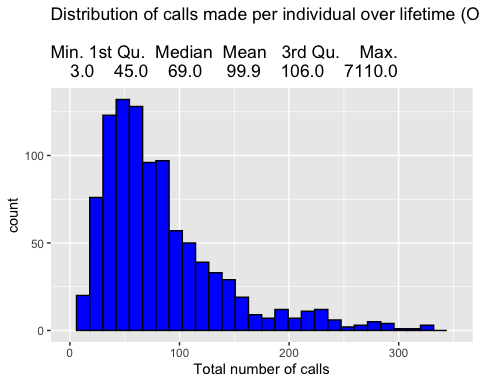
\includegraphics{pad_files/figure-latex/unnamed-chunk-2-3.pdf}

\begin{Shaded}
\begin{Highlighting}[]
\CommentTok{\#Distribution of contenet listened to}

\NormalTok{content\_listened }\OtherTok{\textless{}{-}}\NormalTok{ log\_data }\SpecialCharTok{\%\textgreater{}\%}
  \FunctionTok{group\_by}\NormalTok{(callerId, noContentListened) }\SpecialCharTok{\%\textgreater{}\%}
  \FunctionTok{count}\NormalTok{()}

\CommentTok{\#summary(content\_listened$noContentListened)}

\FunctionTok{ggplot}\NormalTok{(content\_listened, }\FunctionTok{aes}\NormalTok{(}\AttributeTok{x=}\NormalTok{noContentListened)) }\SpecialCharTok{+}
  \FunctionTok{geom\_histogram}\NormalTok{(}\AttributeTok{color=}\StringTok{"black"}\NormalTok{, }\AttributeTok{fill=}\StringTok{"green"}\NormalTok{) }\SpecialCharTok{+}
  \FunctionTok{xlim}\NormalTok{(}\DecValTok{50}\NormalTok{, }\DecValTok{250}\NormalTok{) }\SpecialCharTok{+}
  \FunctionTok{labs}\NormalTok{(}
    \AttributeTok{title =} \StringTok{\textquotesingle{}Distribution of total Content listened to all Across all Calls (Outliers Excluded) }\SpecialCharTok{\textbackslash{}n}
\StringTok{  Min. 1st Qu.  Median  Mean  3rd Qu.    Max. n\textbackslash{}}
\StringTok{  50.00   58.00   74.50   99.97  105.00   2367.00 \textquotesingle{}}\NormalTok{,}
    \AttributeTok{x =} \StringTok{\textquotesingle{}Total Content Listen Across Calls\textquotesingle{}}
\NormalTok{  )}
\end{Highlighting}
\end{Shaded}

\begin{verbatim}
## `stat_bin()` using `bins = 30`. Pick better value with `binwidth`.
\end{verbatim}

\begin{verbatim}
## Warning: Removed 37 rows containing non-finite values (stat_bin).

## Warning: Removed 2 rows containing missing values (geom_bar).
\end{verbatim}

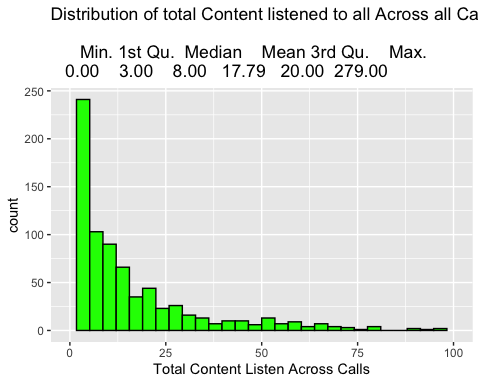
\includegraphics{pad_files/figure-latex/unnamed-chunk-2-4.pdf}

\begin{Shaded}
\begin{Highlighting}[]
\CommentTok{\# Ratio of content per call {-} creating the ratio and graphing the results}
\NormalTok{content\_call\_ratio\_df }\OtherTok{\textless{}{-}} \FunctionTok{inner\_join}\NormalTok{(calls\_made,content\_listened,}\AttributeTok{by=}\StringTok{"callerId"}\NormalTok{)}
\NormalTok{content\_call\_ratio\_df}\SpecialCharTok{$}\NormalTok{ratio }\OtherTok{\textless{}{-}}\NormalTok{ content\_call\_ratio\_df}\SpecialCharTok{$}\NormalTok{noContentListened}\SpecialCharTok{/}\NormalTok{content\_call\_ratio\_df}\SpecialCharTok{$}\NormalTok{noCallsMade}

\CommentTok{\#summary(content\_call\_ratio\_df$ratio)}

\FunctionTok{ggplot}\NormalTok{(content\_call\_ratio\_df, }\FunctionTok{aes}\NormalTok{(}\AttributeTok{x=}\NormalTok{ratio)) }\SpecialCharTok{+}
  \FunctionTok{geom\_histogram}\NormalTok{(}\AttributeTok{color=}\StringTok{"black"}\NormalTok{, }\AttributeTok{fill=}\StringTok{"red"}\NormalTok{) }\SpecialCharTok{+}
  \FunctionTok{xlim}\NormalTok{(}\DecValTok{0}\NormalTok{, }\DecValTok{5}\NormalTok{) }\SpecialCharTok{+}
  \FunctionTok{labs}\NormalTok{(}
    \AttributeTok{title =} \StringTok{\textquotesingle{}Distribution of ratio of content listened to Calls (Outliers Excluded) }\SpecialCharTok{\textbackslash{}n}
\StringTok{    Min.         1st Qu.   Median     Mean    3rd Qu.      Max.}
\StringTok{ 0.05963    0.84598  1.18586  1.40733  1.69773   22.33333  \textquotesingle{}}\NormalTok{,}
    \AttributeTok{x =} \StringTok{\textquotesingle{}Content to Call Ratio\textquotesingle{}}
\NormalTok{  )}
\end{Highlighting}
\end{Shaded}

\begin{verbatim}
## `stat_bin()` using `bins = 30`. Pick better value with `binwidth`.
\end{verbatim}

\begin{verbatim}
## Warning: Removed 11 rows containing non-finite values (stat_bin).

## Warning: Removed 2 rows containing missing values (geom_bar).
\end{verbatim}

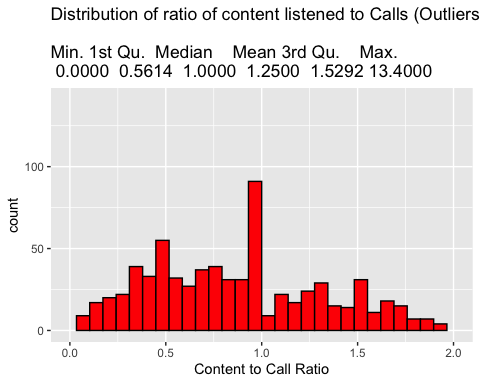
\includegraphics{pad_files/figure-latex/unnamed-chunk-2-5.pdf}

\hypertarget{top-menu}{%
\subsubsection{TOP MENU}\label{top-menu}}

\textbf{Next, we want to Breakd down the initial Menu options and delve
into the distributions of the selections that the farmer can make at a
different state in the IVR System}

\textbf{For the first analysis, we looked at the distribution of the TOP
MENU in the data. This comes in as follows}:

\hypertarget{incoming-call-started-welcome-message-played-assinged-to-experiment-optional-top-menu}{%
\subparagraph{INCOMING CALL STARTED --\textgreater{} WELCOME MESSAGE
PLAYED --\textgreater{} ASSINGED TO EXPERIMENT (OPTIONAL)
--\textgreater{} TOP
MENU}\label{incoming-call-started-welcome-message-played-assinged-to-experiment-optional-top-menu}}

\textbf{TOP MENU}

\begin{itemize}
\tightlist
\item
  RAIN OPTION
\item
  HHI OPTION (household Irrigation)
\item
  RESET PROFILE OPTION
\item
  TOP MENU REPLAY
\item
  LIVESTOCK OPTION
\item
  COVID OPTION
\end{itemize}

\emph{Please note, we are unsure of the order these are presented. For
other menus, we do have the order}

\textbf{Below, we have visualized the number of farmers, out of our
sample, that in the life time of their calling history have accessed a
given TOP MENU item at least once}

\textbf{Additionally, we also visualized this same selection divided by
language to see if the patterns of seleciont are similar or different
across langauges}v

\begin{Shaded}
\begin{Highlighting}[]
\CommentTok{\# filtering out top Menu keys}

\NormalTok{top\_menu }\OtherTok{\textless{}{-}}\FunctionTok{filter}\NormalTok{(log\_data, }\FunctionTok{grepl}\NormalTok{(}\StringTok{"TOP MENU"}\NormalTok{,logInfo))}

\CommentTok{\#cleaning the axis}
\NormalTok{top\_menu}\SpecialCharTok{$}\NormalTok{logInfo}\OtherTok{\textless{}{-}} \FunctionTok{str\_replace}\NormalTok{(top\_menu}\SpecialCharTok{$}\NormalTok{logInfo, }\StringTok{"TOP MENU {-} "}\NormalTok{, }\StringTok{""}\NormalTok{)}
\NormalTok{top\_menu}\SpecialCharTok{$}\NormalTok{logInfo}\OtherTok{\textless{}{-}} \FunctionTok{str\_replace}\NormalTok{(top\_menu}\SpecialCharTok{$}\NormalTok{logInfo, }\StringTok{" PRESSED"}\NormalTok{, }\StringTok{""}\NormalTok{)}
\NormalTok{top\_menu}\SpecialCharTok{$}\NormalTok{logInfo}\OtherTok{\textless{}{-}} \FunctionTok{str\_replace}\NormalTok{(top\_menu}\SpecialCharTok{$}\NormalTok{logInfo, }\StringTok{" PRESSED"}\NormalTok{, }\StringTok{""}\NormalTok{)}
\NormalTok{top\_menu}\SpecialCharTok{$}\NormalTok{logInfo}\OtherTok{\textless{}{-}} \FunctionTok{str\_replace}\NormalTok{(top\_menu}\SpecialCharTok{$}\NormalTok{logInfo, }\StringTok{" SELECTED"}\NormalTok{, }\StringTok{""}\NormalTok{)}

\NormalTok{top\_menu }\OtherTok{\textless{}{-}}\NormalTok{ top\_menu }\SpecialCharTok{\%\textgreater{}\%}
  \FunctionTok{group\_by}\NormalTok{(callerId, logInfo, langId) }\SpecialCharTok{\%\textgreater{}\%}
  \FunctionTok{count}\NormalTok{()}


\FunctionTok{ggplot}\NormalTok{(top\_menu, }\FunctionTok{aes}\NormalTok{(logInfo)) }\SpecialCharTok{+}
  \FunctionTok{theme}\NormalTok{(}\AttributeTok{axis.text.x =} \FunctionTok{element\_text}\NormalTok{(}\AttributeTok{angle =} \DecValTok{30}\NormalTok{, }\AttributeTok{hjust =}\DecValTok{1}\NormalTok{))}\SpecialCharTok{+}
  \FunctionTok{geom\_bar}\NormalTok{()}\SpecialCharTok{+}
  \FunctionTok{labs}\NormalTok{(}
    \AttributeTok{title =} \StringTok{\textquotesingle{}Distirution of TOP MENU items selected at least once by a unique caller\textquotesingle{}}\NormalTok{,}
    \AttributeTok{x =} \StringTok{\textquotesingle{}TOP MENU options\textquotesingle{}}
\NormalTok{  )}
\end{Highlighting}
\end{Shaded}

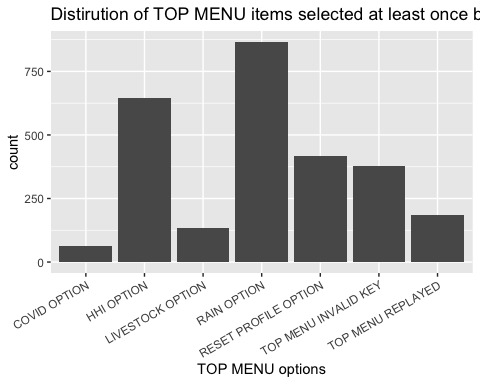
\includegraphics{pad_files/figure-latex/unnamed-chunk-3-1.pdf}

\begin{Shaded}
\begin{Highlighting}[]
\FunctionTok{ggplot}\NormalTok{(top\_menu, }\FunctionTok{aes}\NormalTok{(langId, }\AttributeTok{fill =}\NormalTok{ logInfo)) }\SpecialCharTok{+}
  \FunctionTok{geom\_bar}\NormalTok{()}\SpecialCharTok{+}
  \FunctionTok{labs}\NormalTok{(}
    \AttributeTok{title =} \StringTok{\textquotesingle{}Distirution of Languages divided by TOP MENU option}
\StringTok{    1 = Amharic, 2=Oromiffa, 3=Tigrigna, 4=Wolayitta, and 5=Sidamigna\textquotesingle{}}\NormalTok{,}
    \AttributeTok{x =} \StringTok{\textquotesingle{}Language\textquotesingle{}}
\NormalTok{  )}
\end{Highlighting}
\end{Shaded}

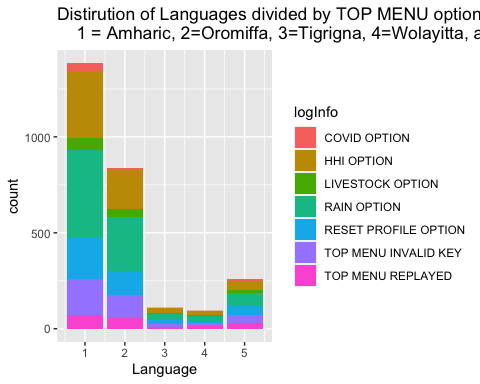
\includegraphics{pad_files/figure-latex/unnamed-chunk-3-2.pdf}

\textbf{As we can easily see, the RAIN options and the HHI option
dominate the choices from the top Menu. So, we decided to dive deeper
into each of these menus to see if there are any outlier selections that
are deep within the system. Additionally, ths distribution across
languages seems to be fairly consistent at face value. We can run tests
in the future, but for EDA this will be adequate. For 3/4 langauge
options - having more data would be apprecaited}

\hypertarget{rain-menu}{%
\subsubsection{RAIN MENU}\label{rain-menu}}

\hypertarget{incoming-call-started-welcome-message-played-random-experiment-top-menu-rain-menu}{%
\subparagraph{INCOMING CALL STARTED --\textgreater{} WELCOME MESSAGE
PLAYED --\textgreater{} RANDOM EXPERIMENT --\textgreater{} TOP MENU
--\textgreater{} RAIN
MENU}\label{incoming-call-started-welcome-message-played-random-experiment-top-menu-rain-menu}}

\textbf{Here, we look at the breakdown of individuals who have selected
a given option in the rain menu at least once. In the data, MAIN MENU ==
RAIN MENU.}

\textbf{RAIN MENU}

\begin{itemize}
\tightlist
\item
  PRE PLANTING OPTION
\item
  PLANTING OPTION
\item
  CROP PROTECTION OPTION
\item
  FERTILIZGER SIDE DREESSING
\item
  POST HARVEST AND PROCESSING
\item
  REPEAT RAIN MENU
\item
  RETURN TO TOP MENU
\item
  INVALID KEY PRESSED (ADDITIONAL OUTCOME)
\end{itemize}

\begin{Shaded}
\begin{Highlighting}[]
\CommentTok{\# Pulling out the rain Menu}

\CommentTok{\#RAIN == HHI\_RAIN}
\NormalTok{rain\_menu }\OtherTok{\textless{}{-}} \FunctionTok{filter}\NormalTok{(log\_data, }\FunctionTok{grepl}\NormalTok{(}\StringTok{"MAIN MENU {-} "}\NormalTok{,logInfo))}
\NormalTok{rain\_menu }\OtherTok{\textless{}{-}} \FunctionTok{filter}\NormalTok{(rain\_menu, }\SpecialCharTok{!}\FunctionTok{grepl}\NormalTok{(}\StringTok{"LIVESTOCK MAIN MENU"}\NormalTok{,logInfo))}
\NormalTok{rain\_menu }\OtherTok{\textless{}{-}} \FunctionTok{filter}\NormalTok{(rain\_menu, }\SpecialCharTok{!}\FunctionTok{grepl}\NormalTok{(}\StringTok{"HHI MAIN MENU"}\NormalTok{,logInfo))}
\NormalTok{rain\_menu }\OtherTok{\textless{}{-}} \FunctionTok{filter}\NormalTok{(rain\_menu, }\SpecialCharTok{!}\FunctionTok{grepl}\NormalTok{(}\StringTok{"COVID{-}19 MAIN MENU"}\NormalTok{,logInfo))}

\CommentTok{\#grouping the observations}
\NormalTok{rain\_menu }\OtherTok{\textless{}{-}}\NormalTok{rain\_menu }\SpecialCharTok{\%\textgreater{}\%}
  \FunctionTok{group\_by}\NormalTok{(callerId, logInfo, langId) }\SpecialCharTok{\%\textgreater{}\%}
  \FunctionTok{count}\NormalTok{()}

\NormalTok{rain\_menu}\SpecialCharTok{$}\NormalTok{logInfo}\OtherTok{\textless{}{-}} \FunctionTok{str\_replace}\NormalTok{(rain\_menu}\SpecialCharTok{$}\NormalTok{logInfo, }\StringTok{"MAIN MENU {-} "}\NormalTok{, }\StringTok{""}\NormalTok{)}
\NormalTok{rain\_menu}\SpecialCharTok{$}\NormalTok{logInfo}\OtherTok{\textless{}{-}} \FunctionTok{str\_replace}\NormalTok{(rain\_menu}\SpecialCharTok{$}\NormalTok{logInfo, }\StringTok{" SELECTED"}\NormalTok{, }\StringTok{""}\NormalTok{)}
\NormalTok{rain\_menu}\SpecialCharTok{$}\NormalTok{logInfo}\OtherTok{\textless{}{-}} \FunctionTok{str\_replace}\NormalTok{(rain\_menu}\SpecialCharTok{$}\NormalTok{logInfo, }\StringTok{" PRESSED"}\NormalTok{, }\StringTok{""}\NormalTok{)}
\NormalTok{rain\_menu}\SpecialCharTok{$}\NormalTok{logInfo}\OtherTok{\textless{}{-}} \FunctionTok{str\_replace}\NormalTok{(rain\_menu}\SpecialCharTok{$}\NormalTok{logInfo, }\StringTok{" OPTION"}\NormalTok{, }\StringTok{""}\NormalTok{)}

\CommentTok{\#plotting rain menu breakdown}
\FunctionTok{ggplot}\NormalTok{(}\AttributeTok{data=}\NormalTok{rain\_menu, }\FunctionTok{aes}\NormalTok{(}\AttributeTok{x=}\NormalTok{logInfo)) }\SpecialCharTok{+}
  \FunctionTok{theme}\NormalTok{(}\AttributeTok{axis.text.x =} \FunctionTok{element\_text}\NormalTok{(}\AttributeTok{angle =} \DecValTok{30}\NormalTok{, }\AttributeTok{hjust =}\DecValTok{1}\NormalTok{))}\SpecialCharTok{+}
  \FunctionTok{geom\_bar}\NormalTok{(}\AttributeTok{fill=}\StringTok{\textquotesingle{}blue\textquotesingle{}}\NormalTok{)}\SpecialCharTok{+}
  \FunctionTok{labs}\NormalTok{(}
    \AttributeTok{title =} \StringTok{\textquotesingle{}Breakdown for Individuals By Content Selected at least Once from the rain menu\textquotesingle{}}\NormalTok{,}
    \AttributeTok{x =} \StringTok{\textquotesingle{}Content Selected\textquotesingle{}}\NormalTok{,}
    \AttributeTok{y=} \StringTok{\textquotesingle{}count\textquotesingle{}}
\NormalTok{  )}
\end{Highlighting}
\end{Shaded}

\includegraphics{pad_files/figure-latex/unnamed-chunk-4-1.pdf}

\textbf{We can see that the pre-planting menu, which still has over 75\%
of unique users accesss it at least once expereinces incredibly high
usage. So, we now dive into this menu. We will breakdown conent
selection by language and overall}

\hypertarget{rain-menupre-planting-menu}{%
\subsubsection{RAIN MENU/PRE PLANTING
MENU}\label{rain-menupre-planting-menu}}

\hypertarget{incoming-call-started-welcome-message-played-random-experiment}{%
\subparagraph{INCOMING CALL STARTED --\textgreater{} WELCOME MESSAGE
PLAYED --\textgreater{} RANDOM EXPERIMENT
--\textgreater{}}\label{incoming-call-started-welcome-message-played-random-experiment}}

\hypertarget{top-menu-rain-menu-pre-planting-menu}{%
\subparagraph{TOP MENU --\textgreater{} RAIN MENU --\textgreater{} PRE
PLANTING MENU}\label{top-menu-rain-menu-pre-planting-menu}}

\textbf{Please note, the pre planting menu under the rain menu is
referred to as MENU 1 in the data}

\textbf{PRE PLANTING MENU}

\begin{itemize}
\tightlist
\item
  LAND PREPARATION
\item
  SEED VARIETY
\item
  REPEAT MENU
\item
  GO TO MAIN MENU (RAIN MENU)
\item
  INVALID KEY (ADDITIONAL OUTCOME)
\end{itemize}

\begin{Shaded}
\begin{Highlighting}[]
\CommentTok{\#filtering out MENU 1 options as the pre planting}
\NormalTok{MENU\_1 }\OtherTok{\textless{}{-}} \FunctionTok{filter}\NormalTok{(log\_data, }\FunctionTok{grepl}\NormalTok{(}\StringTok{"MENU 1"}\NormalTok{,logInfo))}
\NormalTok{MENU\_1 }\OtherTok{\textless{}{-}} \FunctionTok{filter}\NormalTok{(MENU\_1, }\SpecialCharTok{!}\FunctionTok{grepl}\NormalTok{(}\StringTok{"HHIMENU 1"}\NormalTok{,logInfo))}
\NormalTok{MENU\_1 }\OtherTok{\textless{}{-}} \FunctionTok{filter}\NormalTok{(MENU\_1, }\SpecialCharTok{!}\FunctionTok{grepl}\NormalTok{(}\StringTok{"APICULTURE MENU"}\NormalTok{,logInfo))}
\NormalTok{MENU\_1 }\OtherTok{\textless{}{-}} \FunctionTok{filter}\NormalTok{(MENU\_1, }\SpecialCharTok{!}\FunctionTok{grepl}\NormalTok{(}\StringTok{"APICULTURE SUB4 MENU"}\NormalTok{,logInfo))}
\NormalTok{MENU\_1 }\OtherTok{\textless{}{-}} \FunctionTok{filter}\NormalTok{(MENU\_1, }\SpecialCharTok{!}\FunctionTok{grepl}\NormalTok{(}\StringTok{"DAIRY MENU"}\NormalTok{,logInfo))}
\NormalTok{MENU\_1 }\OtherTok{\textless{}{-}} \FunctionTok{filter}\NormalTok{(MENU\_1, }\SpecialCharTok{!}\FunctionTok{grepl}\NormalTok{(}\StringTok{"SMALL{-}SCALE SUB5 MENU"}\NormalTok{,logInfo))}
\NormalTok{MENU\_1 }\OtherTok{\textless{}{-}} \FunctionTok{filter}\NormalTok{(MENU\_1, }\SpecialCharTok{!}\FunctionTok{grepl}\NormalTok{(}\StringTok{"DAIRY SUB2 MENU"}\NormalTok{,logInfo))}
\NormalTok{MENU\_1 }\OtherTok{\textless{}{-}} \FunctionTok{filter}\NormalTok{(MENU\_1, }\SpecialCharTok{!}\FunctionTok{grepl}\NormalTok{(}\StringTok{"FATTENING MANU"}\NormalTok{,logInfo))}

\NormalTok{MENU\_1 }\OtherTok{\textless{}{-}} \FunctionTok{filter}\NormalTok{(MENU\_1, }\SpecialCharTok{!}\FunctionTok{grepl}\NormalTok{(}\StringTok{"FATTENING SUB1 MENU"}\NormalTok{,logInfo))}
\NormalTok{MENU\_1 }\OtherTok{\textless{}{-}} \FunctionTok{filter}\NormalTok{(MENU\_1, }\SpecialCharTok{!}\FunctionTok{grepl}\NormalTok{(}\StringTok{"FATTENING SUB2 MENU"}\NormalTok{,logInfo))}
\NormalTok{MENU\_1 }\OtherTok{\textless{}{-}} \FunctionTok{filter}\NormalTok{(MENU\_1, }\SpecialCharTok{!}\FunctionTok{grepl}\NormalTok{(}\StringTok{"HOUSEHOLD MENU"}\NormalTok{,logInfo))}
\NormalTok{MENU\_1 }\OtherTok{\textless{}{-}} \FunctionTok{filter}\NormalTok{(MENU\_1, }\SpecialCharTok{!}\FunctionTok{grepl}\NormalTok{(}\StringTok{"HOUSEHOLD SUB1 MENU "}\NormalTok{,logInfo))}


\NormalTok{MENU\_1 }\OtherTok{\textless{}{-}}\NormalTok{ MENU\_1 }\SpecialCharTok{\%\textgreater{}\%}
  \FunctionTok{group\_by}\NormalTok{(callerId, logInfo, langId) }\SpecialCharTok{\%\textgreater{}\%}
  \FunctionTok{count}\NormalTok{()}

\NormalTok{MENU\_1}\SpecialCharTok{$}\NormalTok{logInfo}\OtherTok{\textless{}{-}} \FunctionTok{str\_replace}\NormalTok{(MENU\_1}\SpecialCharTok{$}\NormalTok{logInfo, }\StringTok{"MENU 1 {-} "}\NormalTok{, }\StringTok{""}\NormalTok{)}
\NormalTok{MENU\_1}\SpecialCharTok{$}\NormalTok{logInfo}\OtherTok{\textless{}{-}} \FunctionTok{str\_replace}\NormalTok{(MENU\_1}\SpecialCharTok{$}\NormalTok{logInfo, }\StringTok{" PRESSED"}\NormalTok{, }\StringTok{""}\NormalTok{)}
\NormalTok{MENU\_1}\SpecialCharTok{$}\NormalTok{logInfo}\OtherTok{\textless{}{-}} \FunctionTok{str\_replace}\NormalTok{(MENU\_1}\SpecialCharTok{$}\NormalTok{logInfo, }\StringTok{" SELECTED"}\NormalTok{, }\StringTok{""}\NormalTok{)}

\CommentTok{\# plotting}
\FunctionTok{ggplot}\NormalTok{(}\AttributeTok{data=}\NormalTok{MENU\_1, }\FunctionTok{aes}\NormalTok{(}\AttributeTok{x=}\NormalTok{logInfo)) }\SpecialCharTok{+}
  \FunctionTok{theme}\NormalTok{(}\AttributeTok{axis.text.x =} \FunctionTok{element\_text}\NormalTok{(}\AttributeTok{angle =} \DecValTok{25}\NormalTok{, }\AttributeTok{hjust=} \DecValTok{1}\NormalTok{))}\SpecialCharTok{+}
  \FunctionTok{geom\_bar}\NormalTok{(}\AttributeTok{fill=}\StringTok{\textquotesingle{}cyan\textquotesingle{}}\NormalTok{)}\SpecialCharTok{+}
  \FunctionTok{labs}\NormalTok{(}
    \AttributeTok{title =} \StringTok{\textquotesingle{}Individuals By Content Selected at least Once from }
\StringTok{    RAIN MENU/PRE PLANTING OPTION\textquotesingle{}}\NormalTok{,}
    \AttributeTok{x =} \StringTok{\textquotesingle{}Content Selected\textquotesingle{}}\NormalTok{,}
    \AttributeTok{y=} \StringTok{\textquotesingle{}count\textquotesingle{}}
\NormalTok{  )}
\end{Highlighting}
\end{Shaded}

\includegraphics{pad_files/figure-latex/unnamed-chunk-5-1.pdf}

\hypertarget{rain-menupre-planting-menuland-preparation}{%
\subsubsection{RAIN MENU/PRE PLANTING MENU/LAND
PREPARATION}\label{rain-menupre-planting-menuland-preparation}}

\textbf{We continue our pattern of following the most accessed submenu
from the previous subment - land preparation! This is also the bottom of
a tree. We will breakdown conent selection by language and overall}

\hypertarget{incoming-call-started-welcome-message-played-random-experiment-1}{%
\subparagraph{INCOMING CALL STARTED --\textgreater{} WELCOME MESSAGE
PLAYED --\textgreater{} RANDOM EXPERIMENT
--\textgreater{}}\label{incoming-call-started-welcome-message-played-random-experiment-1}}

\hypertarget{top-menu-rain-menu-pre-planting-menu-land-preparation}{%
\subparagraph{TOP MENU --\textgreater{} RAIN MENU --\textgreater{} PRE
PLANTING MENU --\textgreater{} LAND
PREPARATION}\label{top-menu-rain-menu-pre-planting-menu-land-preparation}}

\textbf{LAND PREPARATION}

\begin{itemize}
\tightlist
\item
  BARLEY
\item
  MAIZE
\item
  SORGHUM
\item
  TEF
\item
  WHEAT
\item
  SESAME
\item
  FAVA BEAN
\item
  CHICKPEA
\item
  COMMON BEAN
\item
  COTTON
\end{itemize}

ORDER UNKOWN:

\begin{itemize}
\tightlist
\item
  RICE
\item
  DURAME WHEAT
\item
  LENTIL
\item
  MALT BARLEY
\end{itemize}

\begin{Shaded}
\begin{Highlighting}[]
\CommentTok{\#GETTING THE CROP MENU FROM MENU 1 (rain/preplanting/land preparation sub menu)}
\NormalTok{land\_prep }\OtherTok{\textless{}{-}} \FunctionTok{filter}\NormalTok{(log\_data, }\FunctionTok{grepl}\NormalTok{(}\StringTok{"CONTENT PLAYED {-} LAND PREPARATION {-} "}\NormalTok{,logInfo))}

\NormalTok{land\_prep\_final }\OtherTok{\textless{}{-}}\NormalTok{ land\_prep }\SpecialCharTok{\%\textgreater{}\%}
  \FunctionTok{group\_by}\NormalTok{(callerId, logInfo, langId) }\SpecialCharTok{\%\textgreater{}\%}
  \FunctionTok{count}\NormalTok{()}

\NormalTok{land\_prep\_final}\SpecialCharTok{$}\NormalTok{logInfo}\OtherTok{\textless{}{-}} \FunctionTok{str\_replace}\NormalTok{(land\_prep\_final}\SpecialCharTok{$}\NormalTok{logInfo, }\StringTok{"CONTENT PLAYED {-} LAND PREPARATION {-}"}\NormalTok{, }\StringTok{""}\NormalTok{)}

\FunctionTok{ggplot}\NormalTok{(}\AttributeTok{data=}\NormalTok{land\_prep\_final, }\FunctionTok{aes}\NormalTok{(}\AttributeTok{x=}\NormalTok{logInfo)) }\SpecialCharTok{+}
  \FunctionTok{theme}\NormalTok{(}\AttributeTok{axis.text.x =} \FunctionTok{element\_text}\NormalTok{(}\AttributeTok{angle =} \DecValTok{45}\NormalTok{, }\AttributeTok{hjust=}\DecValTok{1}\NormalTok{))}\SpecialCharTok{+}
  \FunctionTok{geom\_bar}\NormalTok{()}\SpecialCharTok{+}
  \FunctionTok{labs}\NormalTok{(}
    \AttributeTok{title =} \StringTok{\textquotesingle{}RAIN MENU/PRE PLANTING/LAND PREPARATION}
\StringTok{    content actually played by language\textquotesingle{}}\NormalTok{,}
    \AttributeTok{x =} \StringTok{\textquotesingle{}Content Played\textquotesingle{}}\NormalTok{,}
    \AttributeTok{y=} \StringTok{\textquotesingle{}count\textquotesingle{}}
\NormalTok{  )}
\end{Highlighting}
\end{Shaded}

\includegraphics{pad_files/figure-latex/unnamed-chunk-6-1.pdf}

\begin{Shaded}
\begin{Highlighting}[]
\CommentTok{\#get rid of the language breakdown}
\NormalTok{land\_prep\_no\_lang }\OtherTok{\textless{}{-}}\NormalTok{ land\_prep\_final}

\NormalTok{land\_prep\_no\_lang}\SpecialCharTok{$}\NormalTok{logInfo}\OtherTok{\textless{}{-}} \FunctionTok{str\_replace}\NormalTok{(land\_prep\_no\_lang}\SpecialCharTok{$}\NormalTok{logInfo, }\StringTok{"{-} AMHARIC"}\NormalTok{, }\StringTok{""}\NormalTok{)}
\NormalTok{land\_prep\_no\_lang}\SpecialCharTok{$}\NormalTok{logInfo}\OtherTok{\textless{}{-}} \FunctionTok{str\_replace}\NormalTok{(land\_prep\_no\_lang}\SpecialCharTok{$}\NormalTok{logInfo, }\StringTok{"{-} OROMIFFA"}\NormalTok{, }\StringTok{""}\NormalTok{)}
\NormalTok{land\_prep\_no\_lang}\SpecialCharTok{$}\NormalTok{logInfo}\OtherTok{\textless{}{-}} \FunctionTok{str\_replace}\NormalTok{(land\_prep\_no\_lang}\SpecialCharTok{$}\NormalTok{logInfo, }\StringTok{"{-} TIGRIGNA"}\NormalTok{, }\StringTok{""}\NormalTok{)}
\NormalTok{land\_prep\_no\_lang}\SpecialCharTok{$}\NormalTok{logInfo}\OtherTok{\textless{}{-}} \FunctionTok{str\_replace}\NormalTok{(land\_prep\_no\_lang}\SpecialCharTok{$}\NormalTok{logInfo, }\StringTok{"{-} WOLAYITTA"}\NormalTok{, }\StringTok{""}\NormalTok{)}
\NormalTok{land\_prep\_no\_lang}\SpecialCharTok{$}\NormalTok{logInfo}\OtherTok{\textless{}{-}} \FunctionTok{str\_replace}\NormalTok{(land\_prep\_no\_lang}\SpecialCharTok{$}\NormalTok{logInfo, }\StringTok{"{-} WOLAYTIGNA"}\NormalTok{, }\StringTok{""}\NormalTok{)}
\NormalTok{land\_prep\_no\_lang}\SpecialCharTok{$}\NormalTok{logInfo}\OtherTok{\textless{}{-}} \FunctionTok{str\_replace}\NormalTok{(land\_prep\_no\_lang}\SpecialCharTok{$}\NormalTok{logInfo, }\StringTok{"{-} SIDAMIGNA"}\NormalTok{, }\StringTok{""}\NormalTok{)}

\FunctionTok{ggplot}\NormalTok{(land\_prep\_no\_lang, }\FunctionTok{aes}\NormalTok{(}\AttributeTok{x=}\NormalTok{logInfo)) }\SpecialCharTok{+}
  \FunctionTok{theme}\NormalTok{(}\AttributeTok{axis.text.x =} \FunctionTok{element\_text}\NormalTok{(}\AttributeTok{angle =} \DecValTok{90}\NormalTok{))}\SpecialCharTok{+}
  \FunctionTok{geom\_bar}\NormalTok{()}\SpecialCharTok{+}
  \FunctionTok{labs}\NormalTok{(}
    \AttributeTok{title =} \StringTok{\textquotesingle{}RAIN MENU/PRE PLANTING/LAND PREPARATION}
\StringTok{    content played overall\textquotesingle{}}\NormalTok{,}
    \AttributeTok{x =} \StringTok{\textquotesingle{}Content Played\textquotesingle{}}\NormalTok{,}
    \AttributeTok{y=} \StringTok{\textquotesingle{}count\textquotesingle{}}
\NormalTok{  )}
\end{Highlighting}
\end{Shaded}

\includegraphics{pad_files/figure-latex/unnamed-chunk-6-2.pdf}

\begin{Shaded}
\begin{Highlighting}[]
\FunctionTok{ggplot}\NormalTok{(land\_prep\_no\_lang, }\FunctionTok{aes}\NormalTok{(langId, }\AttributeTok{fill =}\NormalTok{ logInfo)) }\SpecialCharTok{+}
  \FunctionTok{geom\_bar}\NormalTok{()}\SpecialCharTok{+}
  \FunctionTok{labs}\NormalTok{(}
    \AttributeTok{title =} \StringTok{\textquotesingle{}ALTERNATIVE RAIN MENU/PRE PLANTING/LAND PREPARATION}
\StringTok{    content actually played by language}
\StringTok{    1 = Amharic, 2=Oromiffa, 3=Tigrigna, 4=Wolayitta, and 5=Sidamigna}
\StringTok{    \textquotesingle{}}\NormalTok{,}
    \AttributeTok{x =} \StringTok{\textquotesingle{}Language\textquotesingle{}}
\NormalTok{  )}
\end{Highlighting}
\end{Shaded}

\includegraphics{pad_files/figure-latex/unnamed-chunk-6-3.pdf}

\textbf{BIG TAKEAWAY: 35\% of users end up accessing the maize menu at
some point! Wheat, Tef, Sorghum, and Barley also appear to be
qualitatively significant}

\textbf{There is no menu to go deeper in, so let's go back up a level
and check to see if other branches have a lot of access}

\hypertarget{rain-menupre-planting-menuseed-variety}{%
\subsubsection{RAIN MENU/PRE PLANTING MENU/SEED
VARIETY}\label{rain-menupre-planting-menuseed-variety}}

\hypertarget{incoming-call-started-welcome-message-played-random-experiment-2}{%
\subparagraph{INCOMING CALL STARTED --\textgreater{} WELCOME MESSAGE
PLAYED --\textgreater{} RANDOM EXPERIMENT
--\textgreater{}}\label{incoming-call-started-welcome-message-played-random-experiment-2}}

\hypertarget{top-menu-rain-menu-pre-planting-menu-seed-variety}{%
\subparagraph{TOP MENU --\textgreater{} RAIN MENU --\textgreater{} PRE
PLANTING MENU --\textgreater{} SEED
VARIETY}\label{top-menu-rain-menu-pre-planting-menu-seed-variety}}

\textbf{SEED VARIETY}

\begin{itemize}
\tightlist
\item
  BARLEY
\item
  MAIZE
\item
  SORGHUM
\item
  TEF
\item
  WHEAT
\item
  SESAME
\item
  FAVA BEAN
\item
  CHICKPEA
\item
  COMMON BEAN
\end{itemize}

\begin{Shaded}
\begin{Highlighting}[]
\CommentTok{\#GETTING THE CROP MENU FROM MENU 1 (rain/preplanting/seed variety sub menu)}
\NormalTok{seed\_variety }\OtherTok{\textless{}{-}} \FunctionTok{filter}\NormalTok{(log\_data, }\FunctionTok{grepl}\NormalTok{(}\StringTok{"CONTENT PLAYED {-} SEED VARITY {-} "}\NormalTok{,logInfo))}

\NormalTok{seed\_variety\_final }\OtherTok{\textless{}{-}}\NormalTok{ seed\_variety }\SpecialCharTok{\%\textgreater{}\%}
  \FunctionTok{group\_by}\NormalTok{(callerId, logInfo, langId) }\SpecialCharTok{\%\textgreater{}\%}
  \FunctionTok{count}\NormalTok{()}

\NormalTok{seed\_variety\_final}\SpecialCharTok{$}\NormalTok{logInfo}\OtherTok{\textless{}{-}} \FunctionTok{str\_replace}\NormalTok{(seed\_variety\_final}\SpecialCharTok{$}\NormalTok{logInfo, }\StringTok{"CONTENT PLAYED {-} SEED VARITY {-} "}\NormalTok{, }\StringTok{""}\NormalTok{)}

\FunctionTok{ggplot}\NormalTok{(}\AttributeTok{data=}\NormalTok{seed\_variety\_final, }\FunctionTok{aes}\NormalTok{(}\AttributeTok{x=}\NormalTok{logInfo)) }\SpecialCharTok{+}
  \FunctionTok{theme}\NormalTok{(}\AttributeTok{axis.text.x =} \FunctionTok{element\_text}\NormalTok{(}\AttributeTok{angle =} \DecValTok{45}\NormalTok{, }\AttributeTok{hjust=}\DecValTok{1}\NormalTok{))}\SpecialCharTok{+}
  \FunctionTok{geom\_bar}\NormalTok{()}\SpecialCharTok{+}
  \FunctionTok{labs}\NormalTok{(}
    \AttributeTok{title =} \StringTok{\textquotesingle{}RAIN MENU/PRE PLANTING/SEED VARIETY}
\StringTok{    content actually played by language\textquotesingle{}}\NormalTok{,}
    \AttributeTok{x =} \StringTok{\textquotesingle{}Content Selected\textquotesingle{}}\NormalTok{,}
    \AttributeTok{y=} \StringTok{\textquotesingle{}count\textquotesingle{}}
\NormalTok{  )}
\end{Highlighting}
\end{Shaded}

\includegraphics{pad_files/figure-latex/unnamed-chunk-7-1.pdf}

\begin{Shaded}
\begin{Highlighting}[]
\CommentTok{\#get rid of the language breakdown}
\NormalTok{seed\_variety\_no\_lang }\OtherTok{\textless{}{-}}\NormalTok{ seed\_variety\_final}

\NormalTok{seed\_variety\_no\_lang}\SpecialCharTok{$}\NormalTok{logInfo}\OtherTok{\textless{}{-}} \FunctionTok{str\_replace}\NormalTok{(seed\_variety\_no\_lang}\SpecialCharTok{$}\NormalTok{logInfo, }\StringTok{"{-} AMHARIC"}\NormalTok{, }\StringTok{""}\NormalTok{)}
\NormalTok{seed\_variety\_no\_lang}\SpecialCharTok{$}\NormalTok{logInfo}\OtherTok{\textless{}{-}} \FunctionTok{str\_replace}\NormalTok{(seed\_variety\_no\_lang}\SpecialCharTok{$}\NormalTok{logInfo, }\StringTok{"{-} OROMIFFA"}\NormalTok{, }\StringTok{""}\NormalTok{)}
\NormalTok{seed\_variety\_no\_lang}\SpecialCharTok{$}\NormalTok{logInfo}\OtherTok{\textless{}{-}} \FunctionTok{str\_replace}\NormalTok{(seed\_variety\_no\_lang}\SpecialCharTok{$}\NormalTok{logInfo, }\StringTok{"{-} TIGRIGNA"}\NormalTok{, }\StringTok{""}\NormalTok{)}
\NormalTok{seed\_variety\_no\_lang}\SpecialCharTok{$}\NormalTok{logInfo}\OtherTok{\textless{}{-}} \FunctionTok{str\_replace}\NormalTok{(seed\_variety\_no\_lang}\SpecialCharTok{$}\NormalTok{logInfo, }\StringTok{"{-} WOLAYITTA"}\NormalTok{, }\StringTok{""}\NormalTok{)}
\NormalTok{seed\_variety\_no\_lang}\SpecialCharTok{$}\NormalTok{logInfo}\OtherTok{\textless{}{-}} \FunctionTok{str\_replace}\NormalTok{(seed\_variety\_no\_lang}\SpecialCharTok{$}\NormalTok{logInfo, }\StringTok{"{-} WOLAYTIGNA"}\NormalTok{, }\StringTok{""}\NormalTok{)}
\NormalTok{seed\_variety\_no\_lang}\SpecialCharTok{$}\NormalTok{logInfo}\OtherTok{\textless{}{-}} \FunctionTok{str\_replace}\NormalTok{(seed\_variety\_no\_lang}\SpecialCharTok{$}\NormalTok{logInfo, }\StringTok{"{-} SIDAMIGNA"}\NormalTok{, }\StringTok{""}\NormalTok{)}

\CommentTok{\#alternative with langauge view}
\FunctionTok{ggplot}\NormalTok{(seed\_variety\_no\_lang, }\FunctionTok{aes}\NormalTok{(langId, }\AttributeTok{fill =}\NormalTok{ logInfo)) }\SpecialCharTok{+}
  \FunctionTok{geom\_bar}\NormalTok{()}\SpecialCharTok{+}
  \FunctionTok{labs}\NormalTok{(}
    \AttributeTok{title =} \StringTok{\textquotesingle{}ALTERNATIVE RAIN MENU/PRE PLANTING/SEE VARIETY}
\StringTok{    content actually played by language}
\StringTok{    1 = Amharic, 2=Oromiffa, 3=Tigrigna, 4=Wolayitta, and 5=Sidamigna}
\StringTok{    \textquotesingle{}}\NormalTok{,}
    \AttributeTok{x =} \StringTok{\textquotesingle{}Language\textquotesingle{}}
\NormalTok{  )}
\end{Highlighting}
\end{Shaded}

\includegraphics{pad_files/figure-latex/unnamed-chunk-7-2.pdf}

\begin{Shaded}
\begin{Highlighting}[]
\CommentTok{\#no language {-} overall}
\FunctionTok{ggplot}\NormalTok{(seed\_variety\_no\_lang, }\FunctionTok{aes}\NormalTok{(}\AttributeTok{x=}\NormalTok{logInfo)) }\SpecialCharTok{+}
  \FunctionTok{theme}\NormalTok{(}\AttributeTok{axis.text.x =} \FunctionTok{element\_text}\NormalTok{(}\AttributeTok{angle =} \DecValTok{30}\NormalTok{, }\AttributeTok{hjust=}\DecValTok{1}\NormalTok{))}\SpecialCharTok{+}
  \FunctionTok{geom\_bar}\NormalTok{()}\SpecialCharTok{+}
  \FunctionTok{labs}\NormalTok{(}
    \AttributeTok{title =} \StringTok{\textquotesingle{}RAIN MENU/PRE PLANTING/seed variety}
\StringTok{    content actually played\textquotesingle{}}\NormalTok{,}
    \AttributeTok{x =} \StringTok{\textquotesingle{}Content Selected\textquotesingle{}}\NormalTok{,}
    \AttributeTok{y=} \StringTok{\textquotesingle{}count\textquotesingle{}}
\NormalTok{  )}
\end{Highlighting}
\end{Shaded}

\includegraphics{pad_files/figure-latex/unnamed-chunk-7-3.pdf}

\textbf{We have mostly exhausted the pre-planting option menu, and if we
go back up to the original rain menu (aka MAIN MENU), we can see that
planting also has a large porportion of users - over half}

\hypertarget{rain-menuplanting-menu}{%
\subsubsection{RAIN MENU/PLANTING MENU}\label{rain-menuplanting-menu}}

\hypertarget{incoming-call-started-welcome-message-played-random-experiment-3}{%
\subparagraph{INCOMING CALL STARTED --\textgreater{} WELCOME MESSAGE
PLAYED --\textgreater{} RANDOM EXPERIMENT
--\textgreater{}}\label{incoming-call-started-welcome-message-played-random-experiment-3}}

\hypertarget{top-menu-rain-menu-planting-menu}{%
\subparagraph{TOP MENU --\textgreater{} RAIN MENU --\textgreater{}
PLANTING MENU}\label{top-menu-rain-menu-planting-menu}}

\textbf{The planting option as a subsection of the rain option is known
as MENU 2 in the data}

PLANTING MENU

\begin{itemize}
\tightlist
\item
  SEED RATE
\item
  SOIL DEPTH PLANTING
\item
  TRANSPLANTING
\item
  MOISTURE CONSERVATION
\item
  FERTILIZER APPLICATION
\item
  REPLAY MENY
\item
  RETURN TO RAIN MENY
\item
  INVALID KEY (ADDITIONAL OUTCOME)
\end{itemize}

\begin{Shaded}
\begin{Highlighting}[]
\CommentTok{\#PLANTING OPTION {-} second most accessed MENU 2}
\NormalTok{MENU\_2 }\OtherTok{\textless{}{-}} \FunctionTok{filter}\NormalTok{(log\_data, }\FunctionTok{grepl}\NormalTok{(}\StringTok{"MENU 2"}\NormalTok{,logInfo))}
\NormalTok{MENU\_2 }\OtherTok{\textless{}{-}} \FunctionTok{filter}\NormalTok{(MENU\_2, }\SpecialCharTok{!}\FunctionTok{grepl}\NormalTok{(}\StringTok{"HHIMENU 2"}\NormalTok{,logInfo))}
\NormalTok{MENU\_2 }\OtherTok{\textless{}{-}} \FunctionTok{filter}\NormalTok{(MENU\_2, }\SpecialCharTok{!}\FunctionTok{grepl}\NormalTok{(}\StringTok{"APICULTURE MENU"}\NormalTok{,logInfo))}
\NormalTok{MENU\_2 }\OtherTok{\textless{}{-}} \FunctionTok{filter}\NormalTok{(MENU\_2, }\SpecialCharTok{!}\FunctionTok{grepl}\NormalTok{(}\StringTok{"APICULTURE SUB2 MENU"}\NormalTok{,logInfo))}
\NormalTok{MENU\_2 }\OtherTok{\textless{}{-}} \FunctionTok{filter}\NormalTok{(MENU\_2, }\SpecialCharTok{!}\FunctionTok{grepl}\NormalTok{(}\StringTok{"DAIRY MENU"}\NormalTok{,logInfo))}
\NormalTok{MENU\_2 }\OtherTok{\textless{}{-}} \FunctionTok{filter}\NormalTok{(MENU\_2, }\SpecialCharTok{!}\FunctionTok{grepl}\NormalTok{(}\StringTok{"FATTENING MANU"}\NormalTok{,logInfo))}

\NormalTok{MENU\_2 }\OtherTok{\textless{}{-}}\NormalTok{ MENU\_2 }\SpecialCharTok{\%\textgreater{}\%}
  \FunctionTok{group\_by}\NormalTok{(callerId, logInfo, langId) }\SpecialCharTok{\%\textgreater{}\%}
  \FunctionTok{count}\NormalTok{()}

\CommentTok{\#cleaning}
\NormalTok{MENU\_2}\SpecialCharTok{$}\NormalTok{logInfo}\OtherTok{\textless{}{-}} \FunctionTok{str\_replace}\NormalTok{(MENU\_2}\SpecialCharTok{$}\NormalTok{logInfo, }\StringTok{"MENU 2 {-} "}\NormalTok{, }\StringTok{""}\NormalTok{)}
\NormalTok{MENU\_2}\SpecialCharTok{$}\NormalTok{logInfo}\OtherTok{\textless{}{-}} \FunctionTok{str\_replace}\NormalTok{(MENU\_2}\SpecialCharTok{$}\NormalTok{logInfo, }\StringTok{" SELECTED"}\NormalTok{, }\StringTok{""}\NormalTok{)}
\NormalTok{MENU\_2}\SpecialCharTok{$}\NormalTok{logInfo}\OtherTok{\textless{}{-}} \FunctionTok{str\_replace}\NormalTok{(MENU\_2}\SpecialCharTok{$}\NormalTok{logInfo, }\StringTok{" PRESSED"}\NormalTok{, }\StringTok{""}\NormalTok{)}
\NormalTok{MENU\_2}\SpecialCharTok{$}\NormalTok{logInfo}\OtherTok{\textless{}{-}} \FunctionTok{str\_replace}\NormalTok{(MENU\_2}\SpecialCharTok{$}\NormalTok{logInfo, }\StringTok{" OPTION"}\NormalTok{, }\StringTok{""}\NormalTok{)}


\CommentTok{\#plotting}
\FunctionTok{ggplot}\NormalTok{(}\AttributeTok{data=}\NormalTok{MENU\_2, }\FunctionTok{aes}\NormalTok{(}\AttributeTok{x=}\FunctionTok{fct\_infreq}\NormalTok{(logInfo))) }\SpecialCharTok{+}
  \FunctionTok{theme}\NormalTok{(}\AttributeTok{axis.text.x =} \FunctionTok{element\_text}\NormalTok{(}\AttributeTok{angle =} \DecValTok{45}\NormalTok{, }\AttributeTok{hjust=}\DecValTok{1}\NormalTok{))}\SpecialCharTok{+}
  \FunctionTok{geom\_bar}\NormalTok{(}\AttributeTok{fill=}\StringTok{\textquotesingle{}olivedrab\textquotesingle{}}\NormalTok{)}\SpecialCharTok{+}
  \FunctionTok{labs}\NormalTok{(}
    \AttributeTok{title =} \StringTok{\textquotesingle{}Individuals By Content Selected at least Once from }
\StringTok{    RAIN MENU/PLANTING OPTION\textquotesingle{}}\NormalTok{,}
    \AttributeTok{x =} \StringTok{\textquotesingle{}Content Selected\textquotesingle{}}\NormalTok{,}
    \AttributeTok{y=} \StringTok{\textquotesingle{}count\textquotesingle{}}
\NormalTok{  )}
\end{Highlighting}
\end{Shaded}

\includegraphics{pad_files/figure-latex/unnamed-chunk-8-1.pdf}

\textbf{As per usual, we will go into the most common selection: seed
rate!}

\hypertarget{rain-menuplanting-menuseed-rate}{%
\subsubsection{RAIN MENU/PLANTING MENU/SEED
RATE}\label{rain-menuplanting-menuseed-rate}}

\hypertarget{incoming-call-started-welcome-message-played-random-experiment-4}{%
\subparagraph{INCOMING CALL STARTED --\textgreater{} WELCOME MESSAGE
PLAYED --\textgreater{} RANDOM EXPERIMENT
--\textgreater{}}\label{incoming-call-started-welcome-message-played-random-experiment-4}}

\hypertarget{top-menu-rain-menu-planting-menu-seed-rate}{%
\subparagraph{TOP MENU --\textgreater{} RAIN MENU --\textgreater{}
PLANTING MENU --\textgreater{} SEED
RATE}\label{top-menu-rain-menu-planting-menu-seed-rate}}

\textbf{SEED RATE}

\begin{itemize}
\tightlist
\item
  BARLEY
\item
  MAIZE
\item
  SORGHUM
\item
  TEF
\item
  WHEAT
\item
  SESAME
\item
  FAVA BEAN
\item
  CHICKPEA
\item
  COMMON BEAN
\item
  COTTON
\end{itemize}

ORDER UNKOWN:

\begin{itemize}
\tightlist
\item
  RICE
\item
  DURAME WHEAT
\item
  LENTIL
\item
  MALT BARLEY
\end{itemize}

\begin{Shaded}
\begin{Highlighting}[]
\NormalTok{seed\_rate }\OtherTok{\textless{}{-}} \FunctionTok{filter}\NormalTok{(log\_data, }\FunctionTok{grepl}\NormalTok{(}\StringTok{"CONTENT PLAYED {-} SEED RATE"}\NormalTok{,logInfo))}

\NormalTok{seed\_rate\_final }\OtherTok{\textless{}{-}}\NormalTok{ seed\_rate }\SpecialCharTok{\%\textgreater{}\%}
  \FunctionTok{group\_by}\NormalTok{(callerId, logInfo, langId) }\SpecialCharTok{\%\textgreater{}\%}
  \FunctionTok{count}\NormalTok{()}

\NormalTok{seed\_rate\_final}\SpecialCharTok{$}\NormalTok{logInfo}\OtherTok{\textless{}{-}} \FunctionTok{str\_replace}\NormalTok{(seed\_rate\_final}\SpecialCharTok{$}\NormalTok{logInfo, }\StringTok{"CONTENT PLAYED {-} SEED RATE {-}"}\NormalTok{, }\StringTok{""}\NormalTok{)}

\FunctionTok{ggplot}\NormalTok{(}\AttributeTok{data=}\NormalTok{seed\_rate\_final, }\FunctionTok{aes}\NormalTok{(}\AttributeTok{x=}\NormalTok{logInfo)) }\SpecialCharTok{+}
  \FunctionTok{theme}\NormalTok{(}\AttributeTok{axis.text.x =} \FunctionTok{element\_text}\NormalTok{(}\AttributeTok{angle =} \DecValTok{90}\NormalTok{))}\SpecialCharTok{+}
  \FunctionTok{geom\_bar}\NormalTok{()}\SpecialCharTok{+}
  \FunctionTok{labs}\NormalTok{(}
    \AttributeTok{title =} \StringTok{\textquotesingle{}RAIN MENU/PLANTING/SEED RATE}
\StringTok{    content actually played by language\textquotesingle{}}\NormalTok{,}
    \AttributeTok{x =} \StringTok{\textquotesingle{}Content Selected\textquotesingle{}}\NormalTok{,}
    \AttributeTok{y=} \StringTok{\textquotesingle{}count\textquotesingle{}}
\NormalTok{  )}
\end{Highlighting}
\end{Shaded}

\includegraphics{pad_files/figure-latex/unnamed-chunk-9-1.pdf}

\begin{Shaded}
\begin{Highlighting}[]
\CommentTok{\#get rid of the language breakdown}
\NormalTok{seed\_rate\_no\_lang }\OtherTok{\textless{}{-}}\NormalTok{ seed\_rate\_final}

\NormalTok{seed\_rate\_no\_lang}\SpecialCharTok{$}\NormalTok{logInfo}\OtherTok{\textless{}{-}} \FunctionTok{str\_replace}\NormalTok{(seed\_rate\_no\_lang}\SpecialCharTok{$}\NormalTok{logInfo, }\StringTok{"{-} AMHARIC"}\NormalTok{, }\StringTok{""}\NormalTok{)}
\NormalTok{seed\_rate\_no\_lang}\SpecialCharTok{$}\NormalTok{logInfo}\OtherTok{\textless{}{-}} \FunctionTok{str\_replace}\NormalTok{(seed\_rate\_no\_lang}\SpecialCharTok{$}\NormalTok{logInfo, }\StringTok{"{-} OROMIFFA"}\NormalTok{, }\StringTok{""}\NormalTok{)}
\NormalTok{seed\_rate\_no\_lang}\SpecialCharTok{$}\NormalTok{logInfo}\OtherTok{\textless{}{-}} \FunctionTok{str\_replace}\NormalTok{(seed\_rate\_no\_lang}\SpecialCharTok{$}\NormalTok{logInfo, }\StringTok{"{-} TIGRIGNA"}\NormalTok{, }\StringTok{""}\NormalTok{)}
\NormalTok{seed\_rate\_no\_lang}\SpecialCharTok{$}\NormalTok{logInfo}\OtherTok{\textless{}{-}} \FunctionTok{str\_replace}\NormalTok{(seed\_rate\_no\_lang}\SpecialCharTok{$}\NormalTok{logInfo, }\StringTok{"{-} WOLAYITTA"}\NormalTok{, }\StringTok{""}\NormalTok{)}
\NormalTok{seed\_rate\_no\_lang}\SpecialCharTok{$}\NormalTok{logInfo}\OtherTok{\textless{}{-}} \FunctionTok{str\_replace}\NormalTok{(seed\_rate\_no\_lang}\SpecialCharTok{$}\NormalTok{logInfo, }\StringTok{"{-} WOLAYTIGNA"}\NormalTok{, }\StringTok{""}\NormalTok{)}
\NormalTok{seed\_rate\_no\_lang}\SpecialCharTok{$}\NormalTok{logInfo}\OtherTok{\textless{}{-}} \FunctionTok{str\_replace}\NormalTok{(seed\_rate\_no\_lang}\SpecialCharTok{$}\NormalTok{logInfo, }\StringTok{"{-} SIDAMIGNA"}\NormalTok{, }\StringTok{""}\NormalTok{)}

\CommentTok{\#alternative with langauge view}
\FunctionTok{ggplot}\NormalTok{(seed\_rate\_no\_lang, }\FunctionTok{aes}\NormalTok{(langId, }\AttributeTok{fill =}\NormalTok{ logInfo)) }\SpecialCharTok{+}
  \FunctionTok{geom\_bar}\NormalTok{()}\SpecialCharTok{+}
  \FunctionTok{labs}\NormalTok{(}
    \AttributeTok{title =} \StringTok{\textquotesingle{}ALTERNATIVE RAIN MENU/PLANTING/SEED RATE}
\StringTok{    content actually played by language}
\StringTok{    1 = Amharic, 2=Oromiffa, 3=Tigrigna, 4=Wolayitta, and 5=Sidamigna}
\StringTok{    \textquotesingle{}}\NormalTok{,}
    \AttributeTok{x =} \StringTok{\textquotesingle{}Language\textquotesingle{}}
\NormalTok{  )}
\end{Highlighting}
\end{Shaded}

\includegraphics{pad_files/figure-latex/unnamed-chunk-9-2.pdf}

\begin{Shaded}
\begin{Highlighting}[]
\CommentTok{\#no language}
\FunctionTok{ggplot}\NormalTok{(seed\_rate\_no\_lang, }\FunctionTok{aes}\NormalTok{(}\AttributeTok{x=}\NormalTok{logInfo)) }\SpecialCharTok{+}
  \FunctionTok{theme}\NormalTok{(}\AttributeTok{axis.text.x =} \FunctionTok{element\_text}\NormalTok{(}\AttributeTok{angle =} \DecValTok{90}\NormalTok{))}\SpecialCharTok{+}
  \FunctionTok{geom\_bar}\NormalTok{()}\SpecialCharTok{+}
  \FunctionTok{labs}\NormalTok{(}
    \AttributeTok{title =} \StringTok{\textquotesingle{}RAIN MENU/PLANTING/SEED RATE}
\StringTok{    content actually played\textquotesingle{}}\NormalTok{,}
    \AttributeTok{x =} \StringTok{\textquotesingle{}Content Selected\textquotesingle{}}\NormalTok{,}
    \AttributeTok{y=} \StringTok{\textquotesingle{}count\textquotesingle{}}
\NormalTok{  )}
\end{Highlighting}
\end{Shaded}

\includegraphics{pad_files/figure-latex/unnamed-chunk-9-3.pdf}

\begin{Shaded}
\begin{Highlighting}[]
\NormalTok{crop\_menu }\OtherTok{\textless{}{-}}\NormalTok{ log\_data }\SpecialCharTok{\%\textgreater{}\%}
  \FunctionTok{filter}\NormalTok{(}\FunctionTok{grepl}\NormalTok{(}\StringTok{"CROP MENU {-} "}\NormalTok{,logInfo)) }\SpecialCharTok{\%\textgreater{}\%}
  \FunctionTok{filter}\NormalTok{(}\SpecialCharTok{!}\FunctionTok{grepl}\NormalTok{(}\StringTok{"HHI"}\NormalTok{,logInfo)) }\SpecialCharTok{\%\textgreater{}\%}
  \FunctionTok{filter}\NormalTok{(}\SpecialCharTok{!}\FunctionTok{grepl}\NormalTok{(}\StringTok{"REPLAYED"}\NormalTok{,logInfo))}

\NormalTok{crop\_menu }\OtherTok{\textless{}{-}}\NormalTok{ crop\_menu }\SpecialCharTok{\%\textgreater{}\%}
  \FunctionTok{group\_by}\NormalTok{(callerId, logInfo, langId) }\SpecialCharTok{\%\textgreater{}\%}
  \FunctionTok{count}\NormalTok{()}

\NormalTok{crop\_menu}\SpecialCharTok{$}\NormalTok{logInfo}\OtherTok{\textless{}{-}} \FunctionTok{str\_replace}\NormalTok{(crop\_menu}\SpecialCharTok{$}\NormalTok{logInfo, }\StringTok{"CROP MENU {-} "}\NormalTok{, }\StringTok{""}\NormalTok{)}
\NormalTok{crop\_menu}\SpecialCharTok{$}\NormalTok{logInfo}\OtherTok{\textless{}{-}} \FunctionTok{str\_replace}\NormalTok{(crop\_menu}\SpecialCharTok{$}\NormalTok{logInfo, }\StringTok{" SELECTED"}\NormalTok{, }\StringTok{""}\NormalTok{)}
\NormalTok{crop\_menu}\SpecialCharTok{$}\NormalTok{logInfo}\OtherTok{\textless{}{-}} \FunctionTok{str\_replace}\NormalTok{(crop\_menu}\SpecialCharTok{$}\NormalTok{logInfo, }\StringTok{"GO TO"}\NormalTok{, }\StringTok{""}\NormalTok{)}


\FunctionTok{ggplot}\NormalTok{(crop\_menu, }\FunctionTok{aes}\NormalTok{(}\AttributeTok{x=}\NormalTok{logInfo)) }\SpecialCharTok{+}
  \FunctionTok{theme}\NormalTok{(}\AttributeTok{axis.text.x =} \FunctionTok{element\_text}\NormalTok{(}\AttributeTok{angle =} \DecValTok{60}\NormalTok{, }\AttributeTok{hjust =}\DecValTok{1}\NormalTok{, }\AttributeTok{size =} \DecValTok{7}\NormalTok{))}\SpecialCharTok{+}
  \FunctionTok{geom\_bar}\NormalTok{()}\SpecialCharTok{+}
  \FunctionTok{labs}\NormalTok{(}
    \AttributeTok{title =} \StringTok{\textquotesingle{}Crop menu breakdown\textquotesingle{}}\NormalTok{,}
    \AttributeTok{x =} \StringTok{\textquotesingle{}Crops\textquotesingle{}}\NormalTok{,}
    \AttributeTok{y=} \StringTok{\textquotesingle{}count\textquotesingle{}}
\NormalTok{  )}
\end{Highlighting}
\end{Shaded}

\includegraphics{pad_files/figure-latex/unnamed-chunk-10-1.pdf}

\begin{Shaded}
\begin{Highlighting}[]
\FunctionTok{ggplot}\NormalTok{(crop\_menu, }\FunctionTok{aes}\NormalTok{(langId, }\AttributeTok{fill =}\NormalTok{ logInfo)) }\SpecialCharTok{+}
  \FunctionTok{geom\_bar}\NormalTok{()}\SpecialCharTok{+}
  \FunctionTok{labs}\NormalTok{(}
    \AttributeTok{title =} \StringTok{\textquotesingle{}CROP MENU BY LANGUAGE}
\StringTok{    1 = Amharic, 2=Oromiffa, 3=Tigrigna, 4=Wolayitta, and 5=Sidamigna}
\StringTok{    \textquotesingle{}}\NormalTok{,}
    \AttributeTok{x =} \StringTok{\textquotesingle{}Language\textquotesingle{}}
\NormalTok{  )}
\end{Highlighting}
\end{Shaded}

\includegraphics{pad_files/figure-latex/unnamed-chunk-10-2.pdf}

\begin{Shaded}
\begin{Highlighting}[]
\NormalTok{num\_crop\_types }\OtherTok{\textless{}{-}} \FunctionTok{data.frame}\NormalTok{(}\FunctionTok{as.numeric}\NormalTok{(}\FunctionTok{table}\NormalTok{(crop\_menu}\SpecialCharTok{$}\NormalTok{callerId)))}
\NormalTok{num\_crop\_types}\SpecialCharTok{$}\NormalTok{frequencies }\OtherTok{\textless{}{-}}\NormalTok{ num\_crop\_types}\SpecialCharTok{$}\NormalTok{as.numeric.table.crop\_menu.callerId.}

\FunctionTok{summary}\NormalTok{(num\_crop\_types}\SpecialCharTok{$}\NormalTok{frequencies)}
\end{Highlighting}
\end{Shaded}

\begin{verbatim}
##    Min. 1st Qu.  Median    Mean 3rd Qu.    Max. 
##   1.000   2.000   4.000   4.915   7.000  15.000
\end{verbatim}

\begin{Shaded}
\begin{Highlighting}[]
\FunctionTok{ggplot}\NormalTok{(num\_crop\_types, }\FunctionTok{aes}\NormalTok{(frequencies)) }\SpecialCharTok{+}
  \FunctionTok{geom\_histogram}\NormalTok{(}\AttributeTok{color=}\StringTok{"black"}\NormalTok{, }\AttributeTok{fill=}\StringTok{"red"}\NormalTok{) }\SpecialCharTok{+}
  \FunctionTok{labs}\NormalTok{(}
    \AttributeTok{title =} \StringTok{\textquotesingle{}Distribution of number crops ever selected by individual }\SpecialCharTok{\textbackslash{}n}
\StringTok{      Min.  1st Qu.  Median    Mean   3rd Qu.    Max. }
\StringTok{  1.000     2.000     4.000      4.915     7.000     15.000 \textquotesingle{}}\NormalTok{,}
    \AttributeTok{x =} \StringTok{\textquotesingle{}Number of crops selected \textquotesingle{}}
\NormalTok{  )}
\end{Highlighting}
\end{Shaded}

\begin{verbatim}
## `stat_bin()` using `bins = 30`. Pick better value with `binwidth`.
\end{verbatim}

\includegraphics{pad_files/figure-latex/unnamed-chunk-10-3.pdf}

HOW MANY CROPS PER USER ARE LOOKED AT??????????

\end{document}
